\chapter{結果と考察}
共振周波数を変化させるためには、共振器の大きさを変化させる方法と、
内部に誘電体または導体を挿入する方法がある。
共振器自体の大きさを変化させて共振周波数を調整する方法では、
全ての辺の長さの比を一定にしなければ、内部の電磁場分布が大きく変化してしまい、
大きさの変化とともに試料位置も変化させる必要があるが、
試料位置を可変にすることは現実的でない。
また、全ての方向で大きさの比を保ちながら
共振器の大きさを変化させるためにはかなり高度なギミックが必要となり、
これも現実的ではない。
そのため本研究では内部に誘電体を挿入して
共振周波数を減少させる方法くを検討した。


\section{誘電体の挿入効果}
まず、誘電体挿入による共振周波数の変化を検証した。

\vspace{10 mm}

\begin{figure}[h]
  \begin{center}
    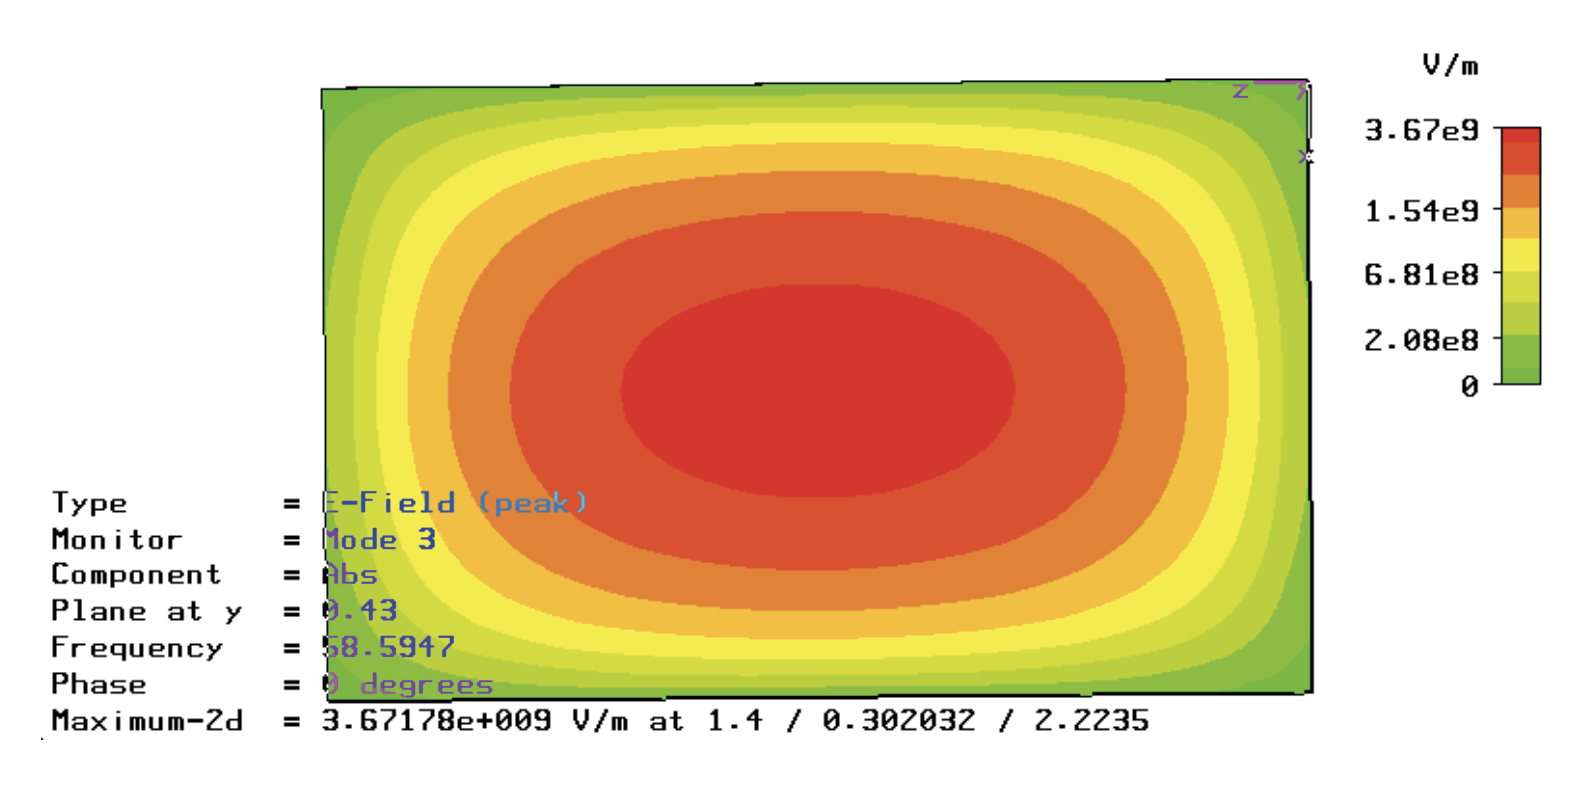
\includegraphics[width=12cm]{./image/te101.png}
    \caption{TE$_{101}$モードの電場振幅の空間分布}
    \label{fig:E-TE101}
  \end{center}
\end{figure}

図4.1 のように基本モードTE$_{101}$を持つ空洞共振器を設計した。
この図では電場分振幅の空間分布を表しており、中心の方が振幅が大きく、
端に向かうにしたがって小さくなっていることがわかる。

この基本モードに対し、誘電率9の誘電体(サファイア)を以下のように変化させる2つのモデルで検証を行った。

\begin{enumerate}
  \item 共振器よりも小さいサイズ(0.5mm)で位置を変化させる。(Fig4.2)
  \item 共振器と同じ長さを持った誘電体を徐々に挿入し空洞に占める誘電体の体積を変化させるモデル。(Fig4.3)
\end{enumerate}

Fig.4.2およびFig.4.3において水色部分が共振器、青色部分が誘電体(サファイア)である。
また、共振器の長さは4.8mmとし、
誘電体の位置は、
% 誘電体の初期位置でもっとも共振器中心に近い面を基準にして検証を行った。

\vspace{10 mm}

\begin{figure}[h]
  \begin{center}
    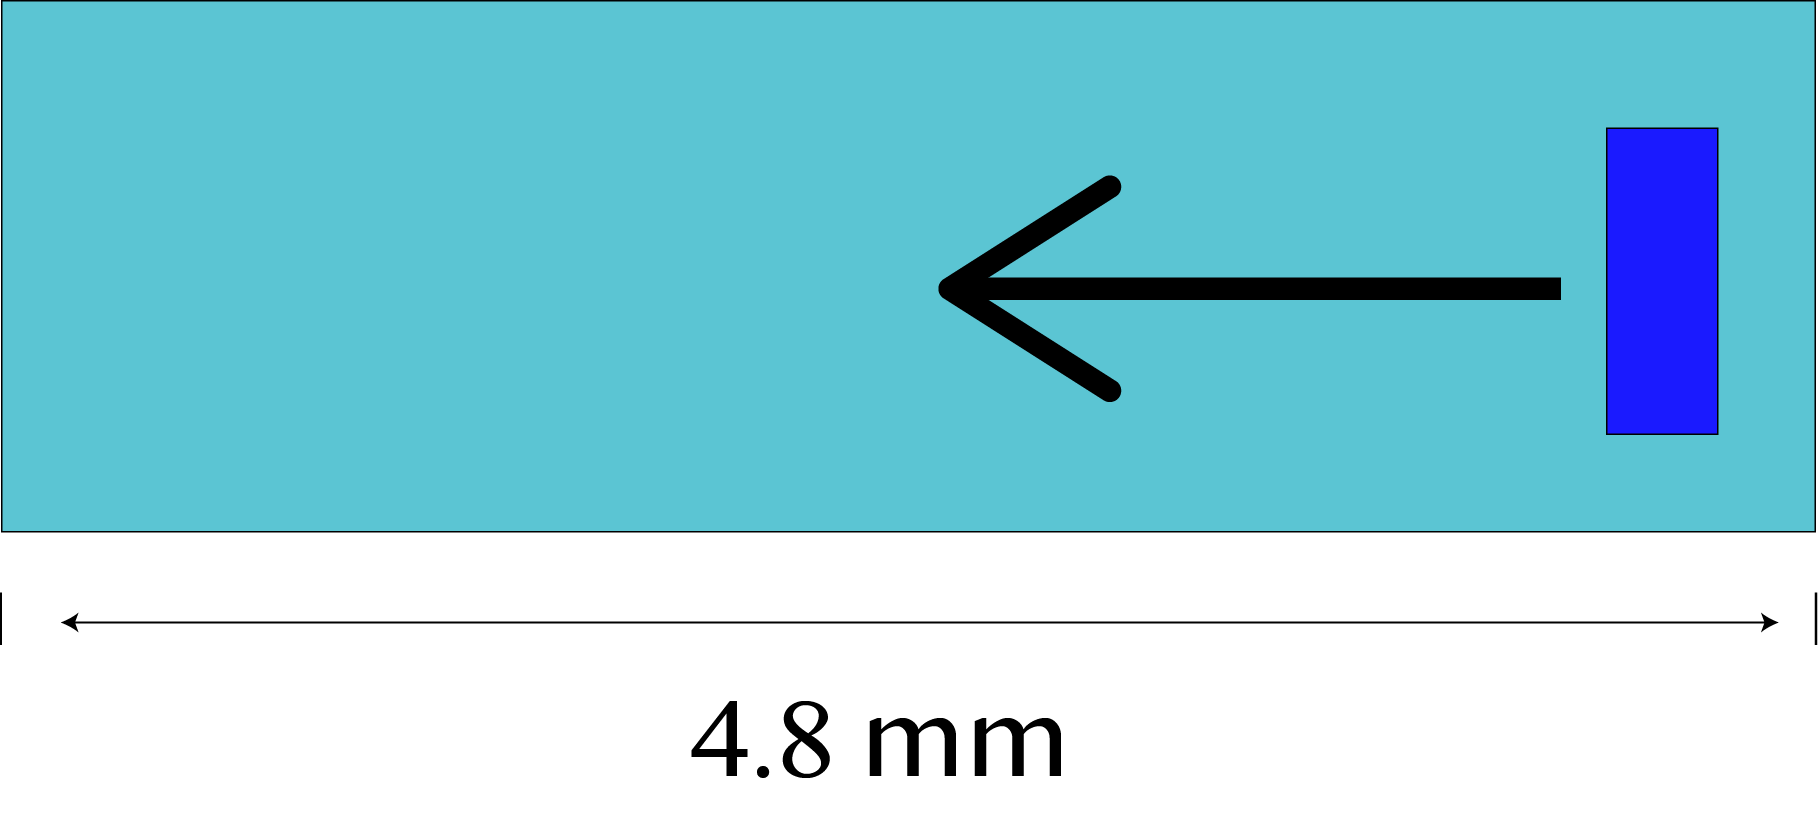
\includegraphics[width=8cm]{./image/pos.png}
    \caption{位置のみを変化させたモデル}
    \label{fig:potition}
  \end{center}
\end{figure}

\vspace{10 mm}

\begin{figure}[h]
  \begin{center}
    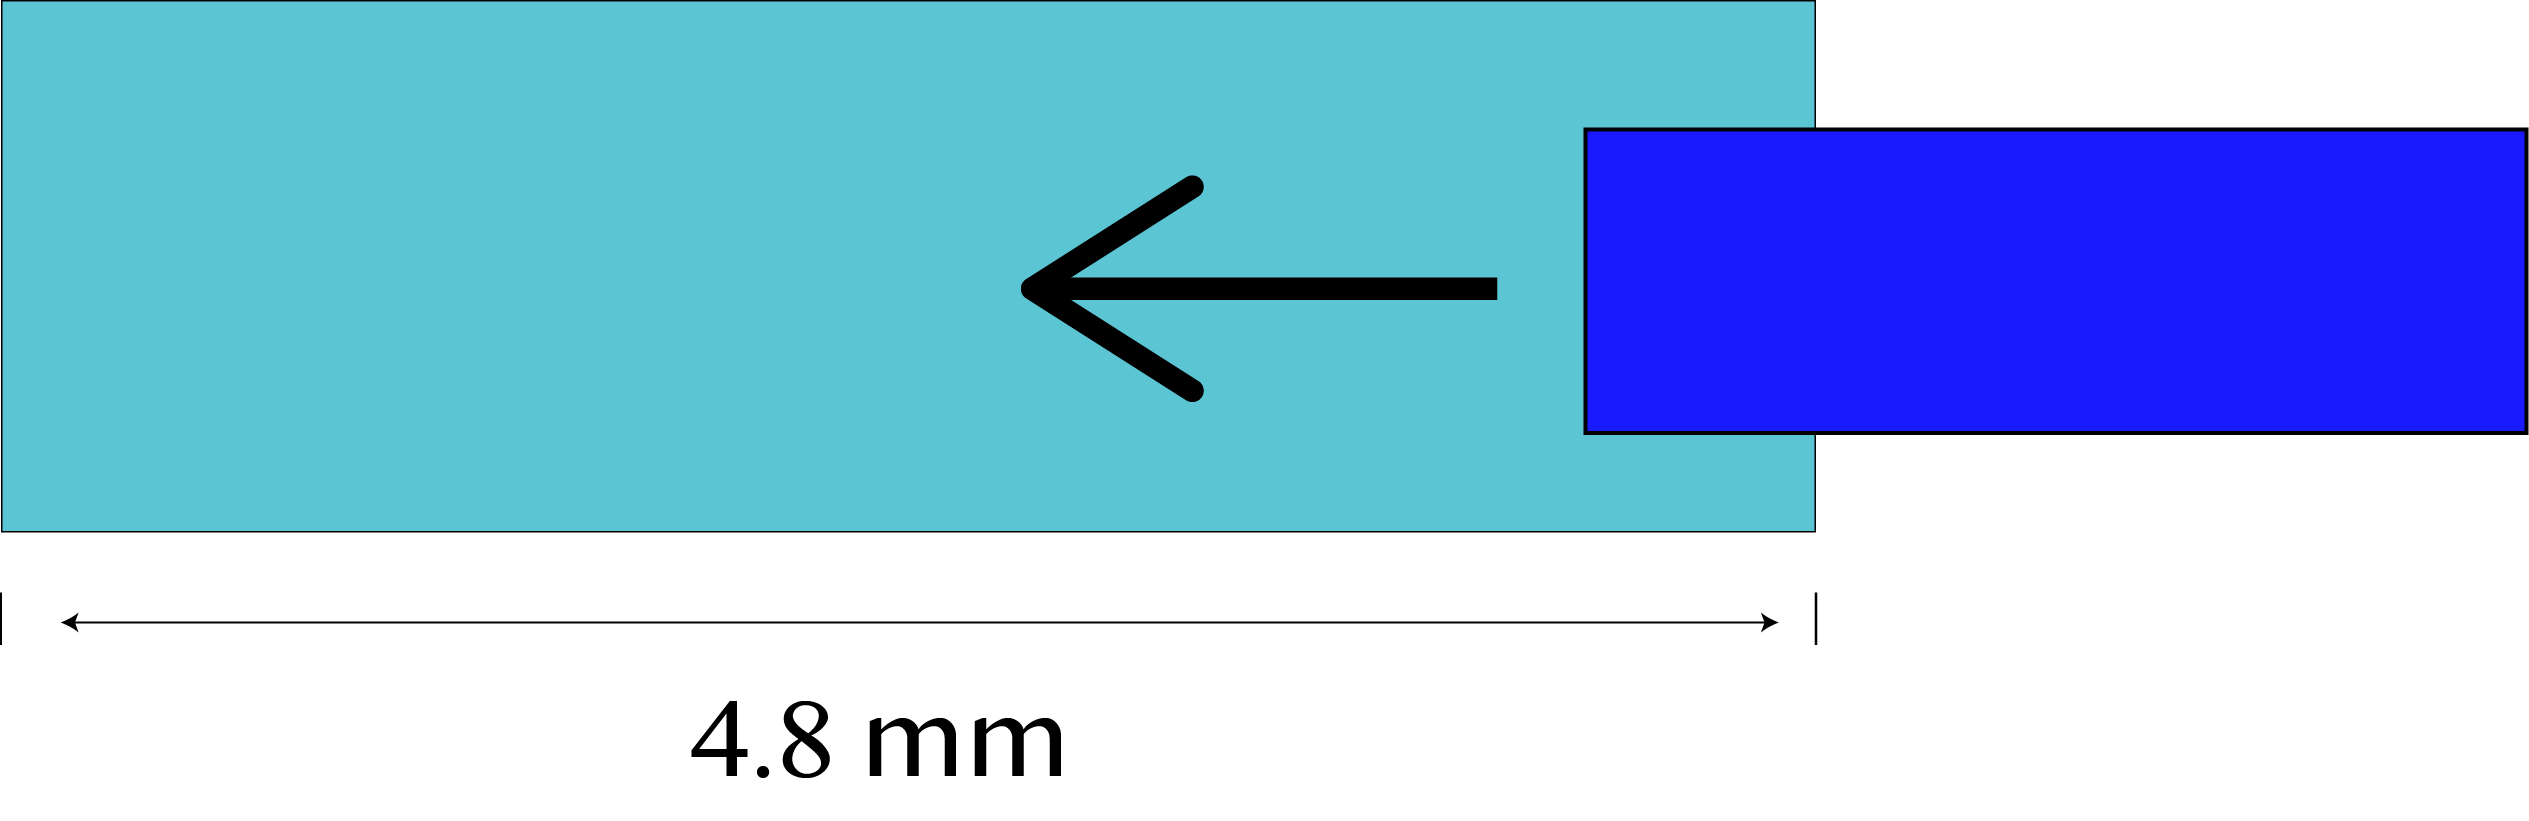
\includegraphics[width=11cm]{./image/length.png}
    \caption{誘電体を挿入していったモデル}
    \label{fig:length}
  \end{center}
\end{figure}

\subsection*{結果}
Fig.4.4に検証結果を示す。
赤で示した点がモデル1の結果であり、青で示した点がモデル2の結果である。
これより、電場振幅の大きい場所に誘電体をおいた方が
共振周波数が変化が大きいこと、
および
モデル1とモデル2では、
変化の最大値はモデル2の方が大きいことがわかった。
また、どちらのモデルも一定の位置($x$〜2mm)まで共振周波数が
変化しなかったことから、
電場振幅の小さい場所に誘電体を挿入しても
共振周波数は変化しないことがわかった。

% モデル1において、共振器の終端に誘電体が到達した点の共振周波数が最初の位置での共振周波数から下がってしまっている。また、その他の点でも中心点から対照的なプロットになっていないように見える。この点については以下で考察を行う。

\vspace{10 mm}

\begin{figure}[h]
  \begin{center}
    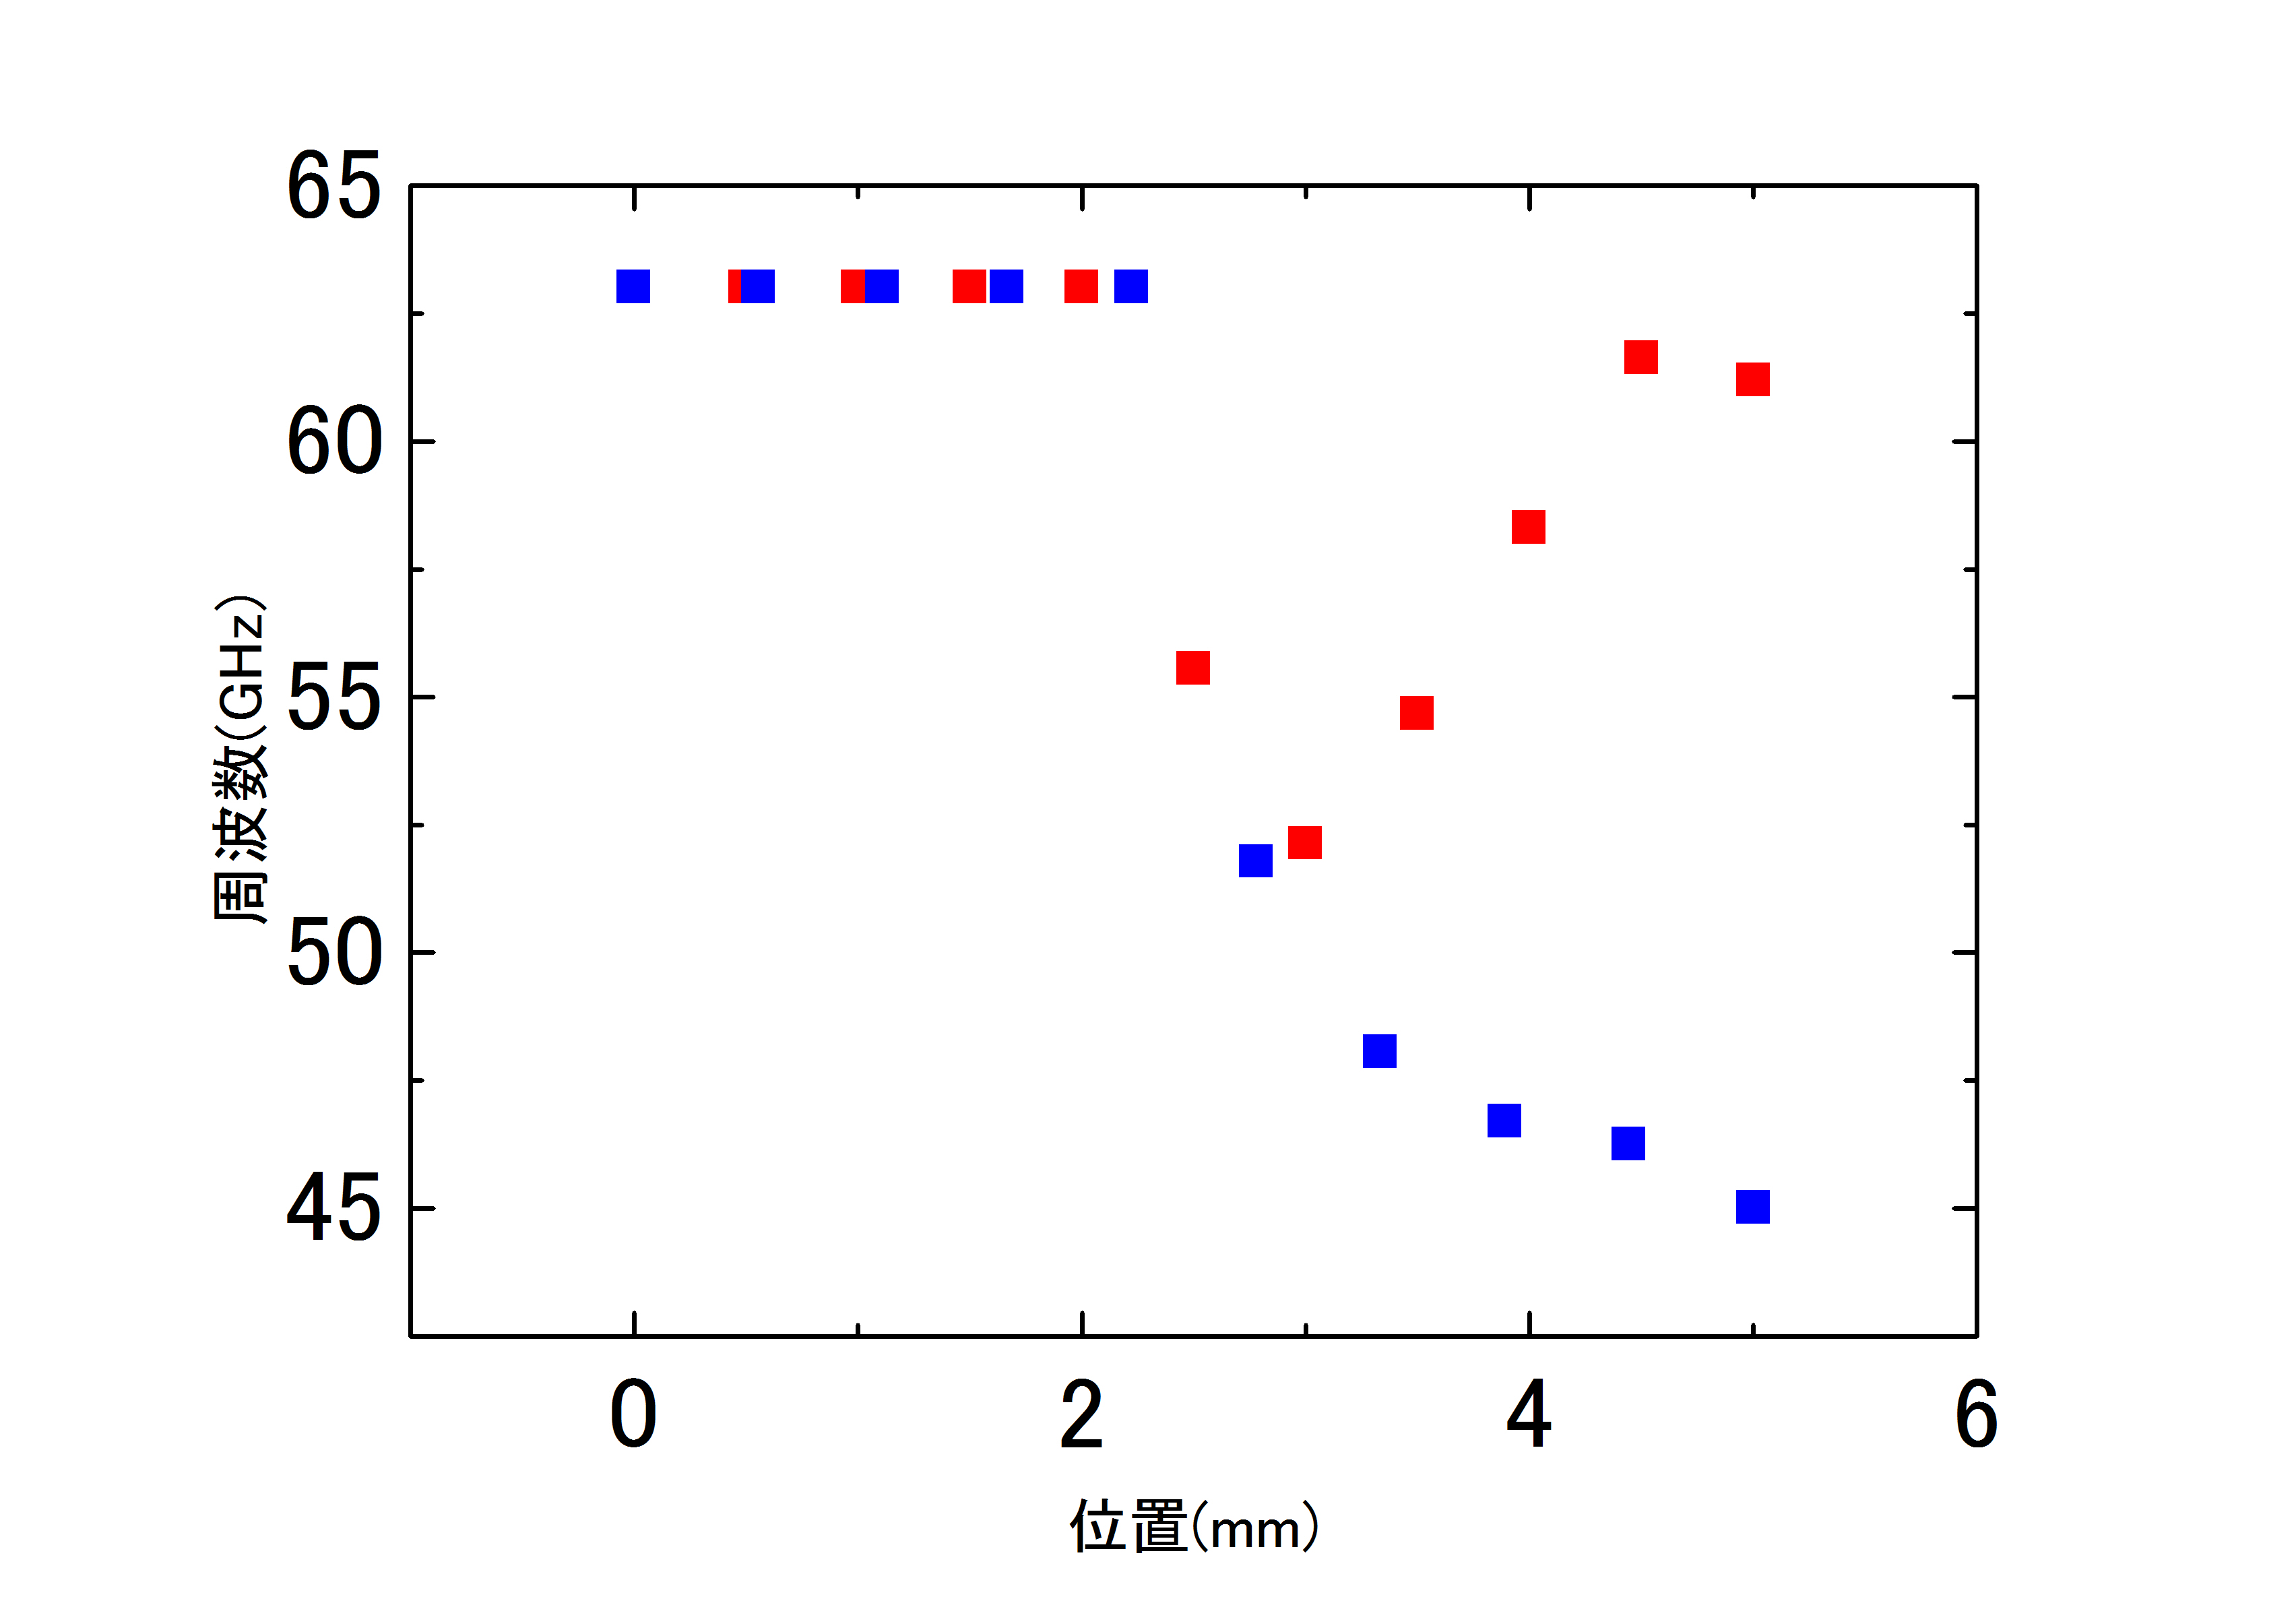
\includegraphics[width=12cm]{./image/plot1.jpg}
    \caption{誘電体による共振周波数の変化の検証}
    \label{fig:Cavity}
  \end{center}
\end{figure}


\subsection*{考察}
位置のみを変えたモデルで最後の点と最初の点での共振周波数が異なっているのは、
共振器の壁に誘電体が到達してしまったことで、
別のモードが発現し、その共振周波数が記録されてしまっているためであると考えられる。

また、対照的なプロットにならなかったのは、
位置座標の取り方が大きく影響していると考えられる。
上記の結果から、誘電体が電場振幅の強い部分に存在する際に、
共振周波数は大きく影響を受ける。
しかし、今回は誘電体の片面を基準にしてしまったために、位置によって、
誘電体のどの程度の部分が電場振幅が強い場所にあるのか、という情報が中心軸を境に、変わってしまった。
以降同様の検証を行う場合には、誘電体の中心を基準点としてとると
対照的なプロットが取れると期待出来る。



これらの結果を受けて、共振周波数を大きく変化させるためには、共振器内部の「電場振幅の大きい場所」に誘電体を「挿入」すると良さそうである。

\section{同軸ケーブルとの結合と試料位置を考慮したモデル}
4.1節に示した計算結果を受けて、Fig4.5とFig4.6に示す
% の基本モード
TE$_{101}$モード、共振周波数$f$=61GHz(固有値解析)の直方型空洞共振器を設計した。

\subsection*{詳細設計}
具体的には、直方型空洞の各辺に平行な互いに直行する
% 独立した
3つの方向をx,y,z方向と呼ぶと
% する。
し、a=2.8mm,b=1.5mm,l=4.8mmで張られる
% 以下で使う長さの単位がmmである場合には省略して表記する
% 基本となる
空洞の大きさを(x,y,z)=(2.8,1.5,4.8)と表す。
共振器の底面中央に
Fig.4.7に示す大きさ(x,y,z)=(2.8,0.5,1.5)の
誘電体基板(サファイヤ)を設置した。
% (図4.7)
Fig.4.5に示すこの基板上に超伝導素子を設置する。
空洞上部中央に共振周波数を調整するための誘電体を
大きさ(x,y,z)=(2.8,0.5,1.5)として挿入した。
これらの誘電体は比誘電率9を持つサファイアを仮定した。
% 誘電体、基盤として用いるサファイアは、
厚みを0.5mmとした理由は、
北野研究室でよく使用されるサファイア基板の厚さが0.5mmであるため
である。
% そこから切り出しやすいように今回使用する厚みも5mmとした。
% 試料の位置は図4.5を参照。
試料用の基盤と共振周波数の調整用誘電体の大きさを同じにしたのは
試料位置における電場を最大にするためである。x
% また過去に行われたcavity-QED実験\cite{cQED}を参考にして、
% 外界との結合のため共振器上部に高さ1mm励振部を設置した。
外部との結合に用いる同軸ケーブルのサイズは先行研究\cite{cQED}を参考に
外部導体の外径$φ$=2.197mm、
内部誘電体層(テフロン:誘電率2)の外径$φ$=1.676mm、
中心導体の外径$φ$=0.511mmとし、
長さ1mmの励振部を設けた。
% また、空洞共振器の壁には完全導体(PEC)を使用し、内部は真空とした。

\vspace{10 mm}

\begin{figure}[h]
  \begin{center}
    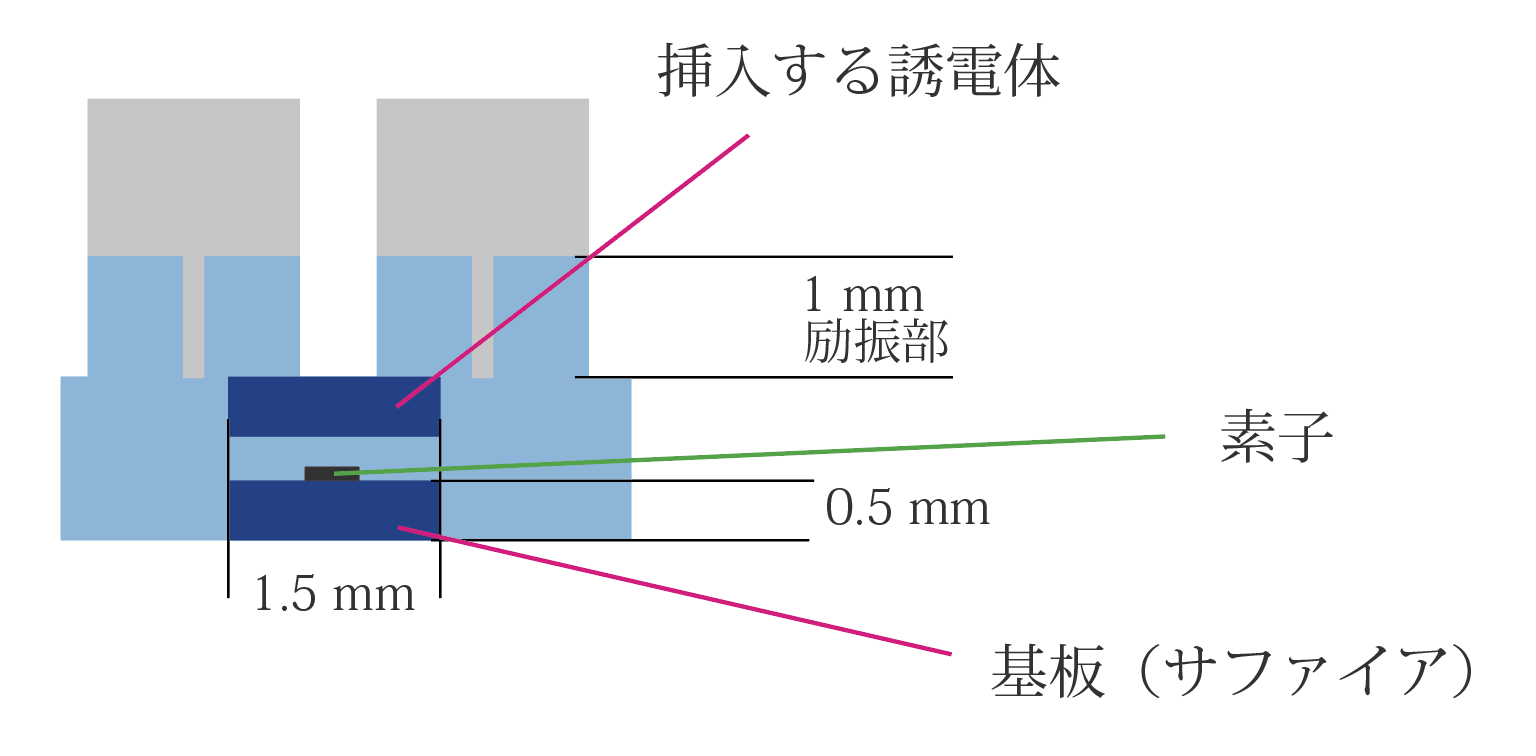
\includegraphics[width=12cm]{./image/newmodel.png}
    \caption{設計したモデルの断面からの図}
    \label{fig:Cavity}
  \end{center}
\end{figure}

\vspace{10 mm}

\begin{figure}[h]
 \begin{minipage}{0.5\hsize}
  \begin{center}
   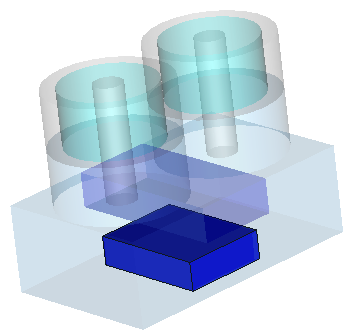
\includegraphics[width=70mm]{./image/model73.png}
  \end{center}
  \caption{設計したモデルの立体図}
  \label{fig:one}
 \end{minipage}
 \begin{minipage}{0.5\hsize}
  \begin{center}
   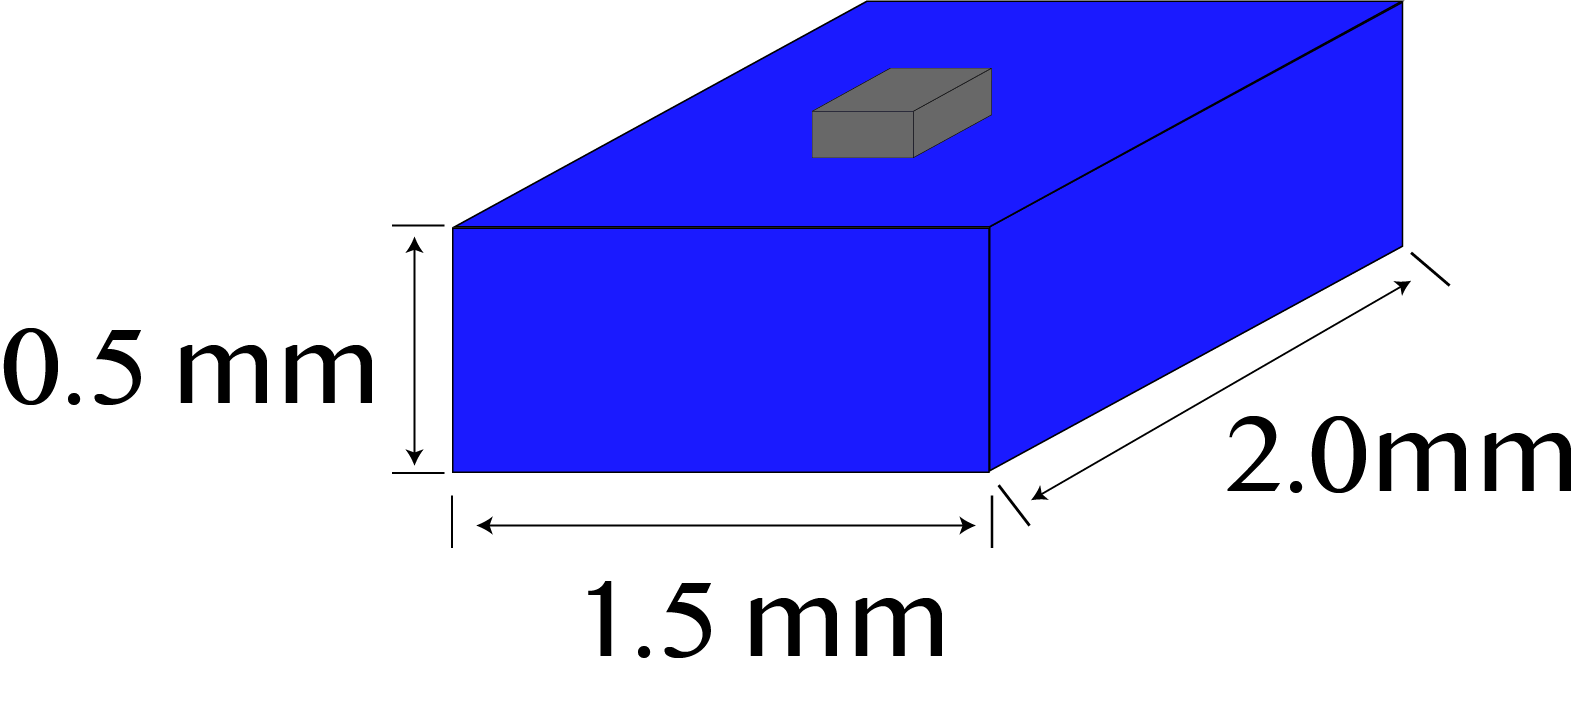
\includegraphics[width=70mm]{./image/基板資料あり.png}
  \end{center}
  \caption{基板に試料を乗せた図}
  \label{fig:two}
 \end{minipage}
\end{figure}

% 実際に実験を行う際には、図4.7にあるように、
% 共振器の底に設置した誘電体の上には超伝導体の試料を載せる。

\subsection*{基本性質}
共振周波数調整用のサファイヤ板を「誘電体」、
試料設置用のサファイアを「基板」と表して、
% 以下に3つの場合の空洞内電場の$y$成分(高さ方向)と共振特性(Sパラメータ)を調べた。
% この共振器の基本的な性質を示す。
% 以下それぞれ、左に固有値解析の結果、右に過渡解析の結果を示す。
% 過渡解析の結果はSパラメータを表示している。
% シミュレーションでは入力ポートと出力ポートを設定しており、
% 下図赤線で示された
Sパラメータのうち、
S$_{11}$は入力電力に対する反射電力比を表し、
% 下図青線で示された
S$_{21}$は入力電力に対する透過電力比を表す。
% その2つの値が大きく逆向きに変動している場所で共振していると言える。


\subsubsection{誘電体なし基板なし}
まず、誘電体も基板も設置していない場合の解析結果
% は以下のようになっている。
をFig.4.8とFig.4.9に示す。
過渡解析の結果、狙ったモード(TE$_{101}$)での共振が観測された。
前述の基板や誘電体の場所はこの結果に基づいて、決定した。

\begin{figure}[h]
 \begin{minipage}{0.5\hsize}
  \begin{center}
   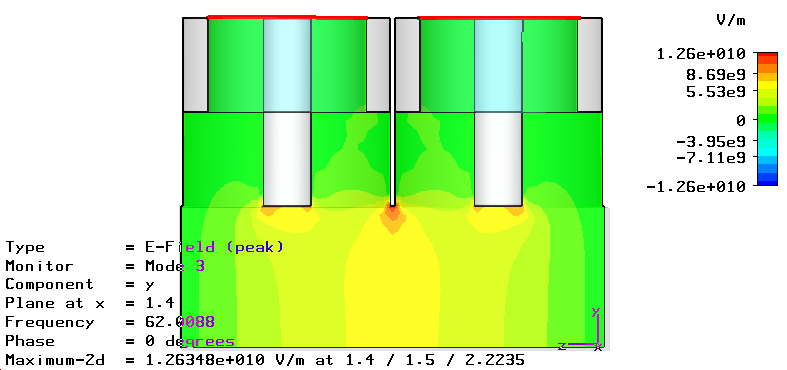
\includegraphics[width=70mm]{./image/model73_vac.png}
  \end{center}
  \caption{E$_y$の空間分布}
  \label{fig:one}
 \end{minipage}
 \begin{minipage}{0.5\hsize}
  \begin{center}
   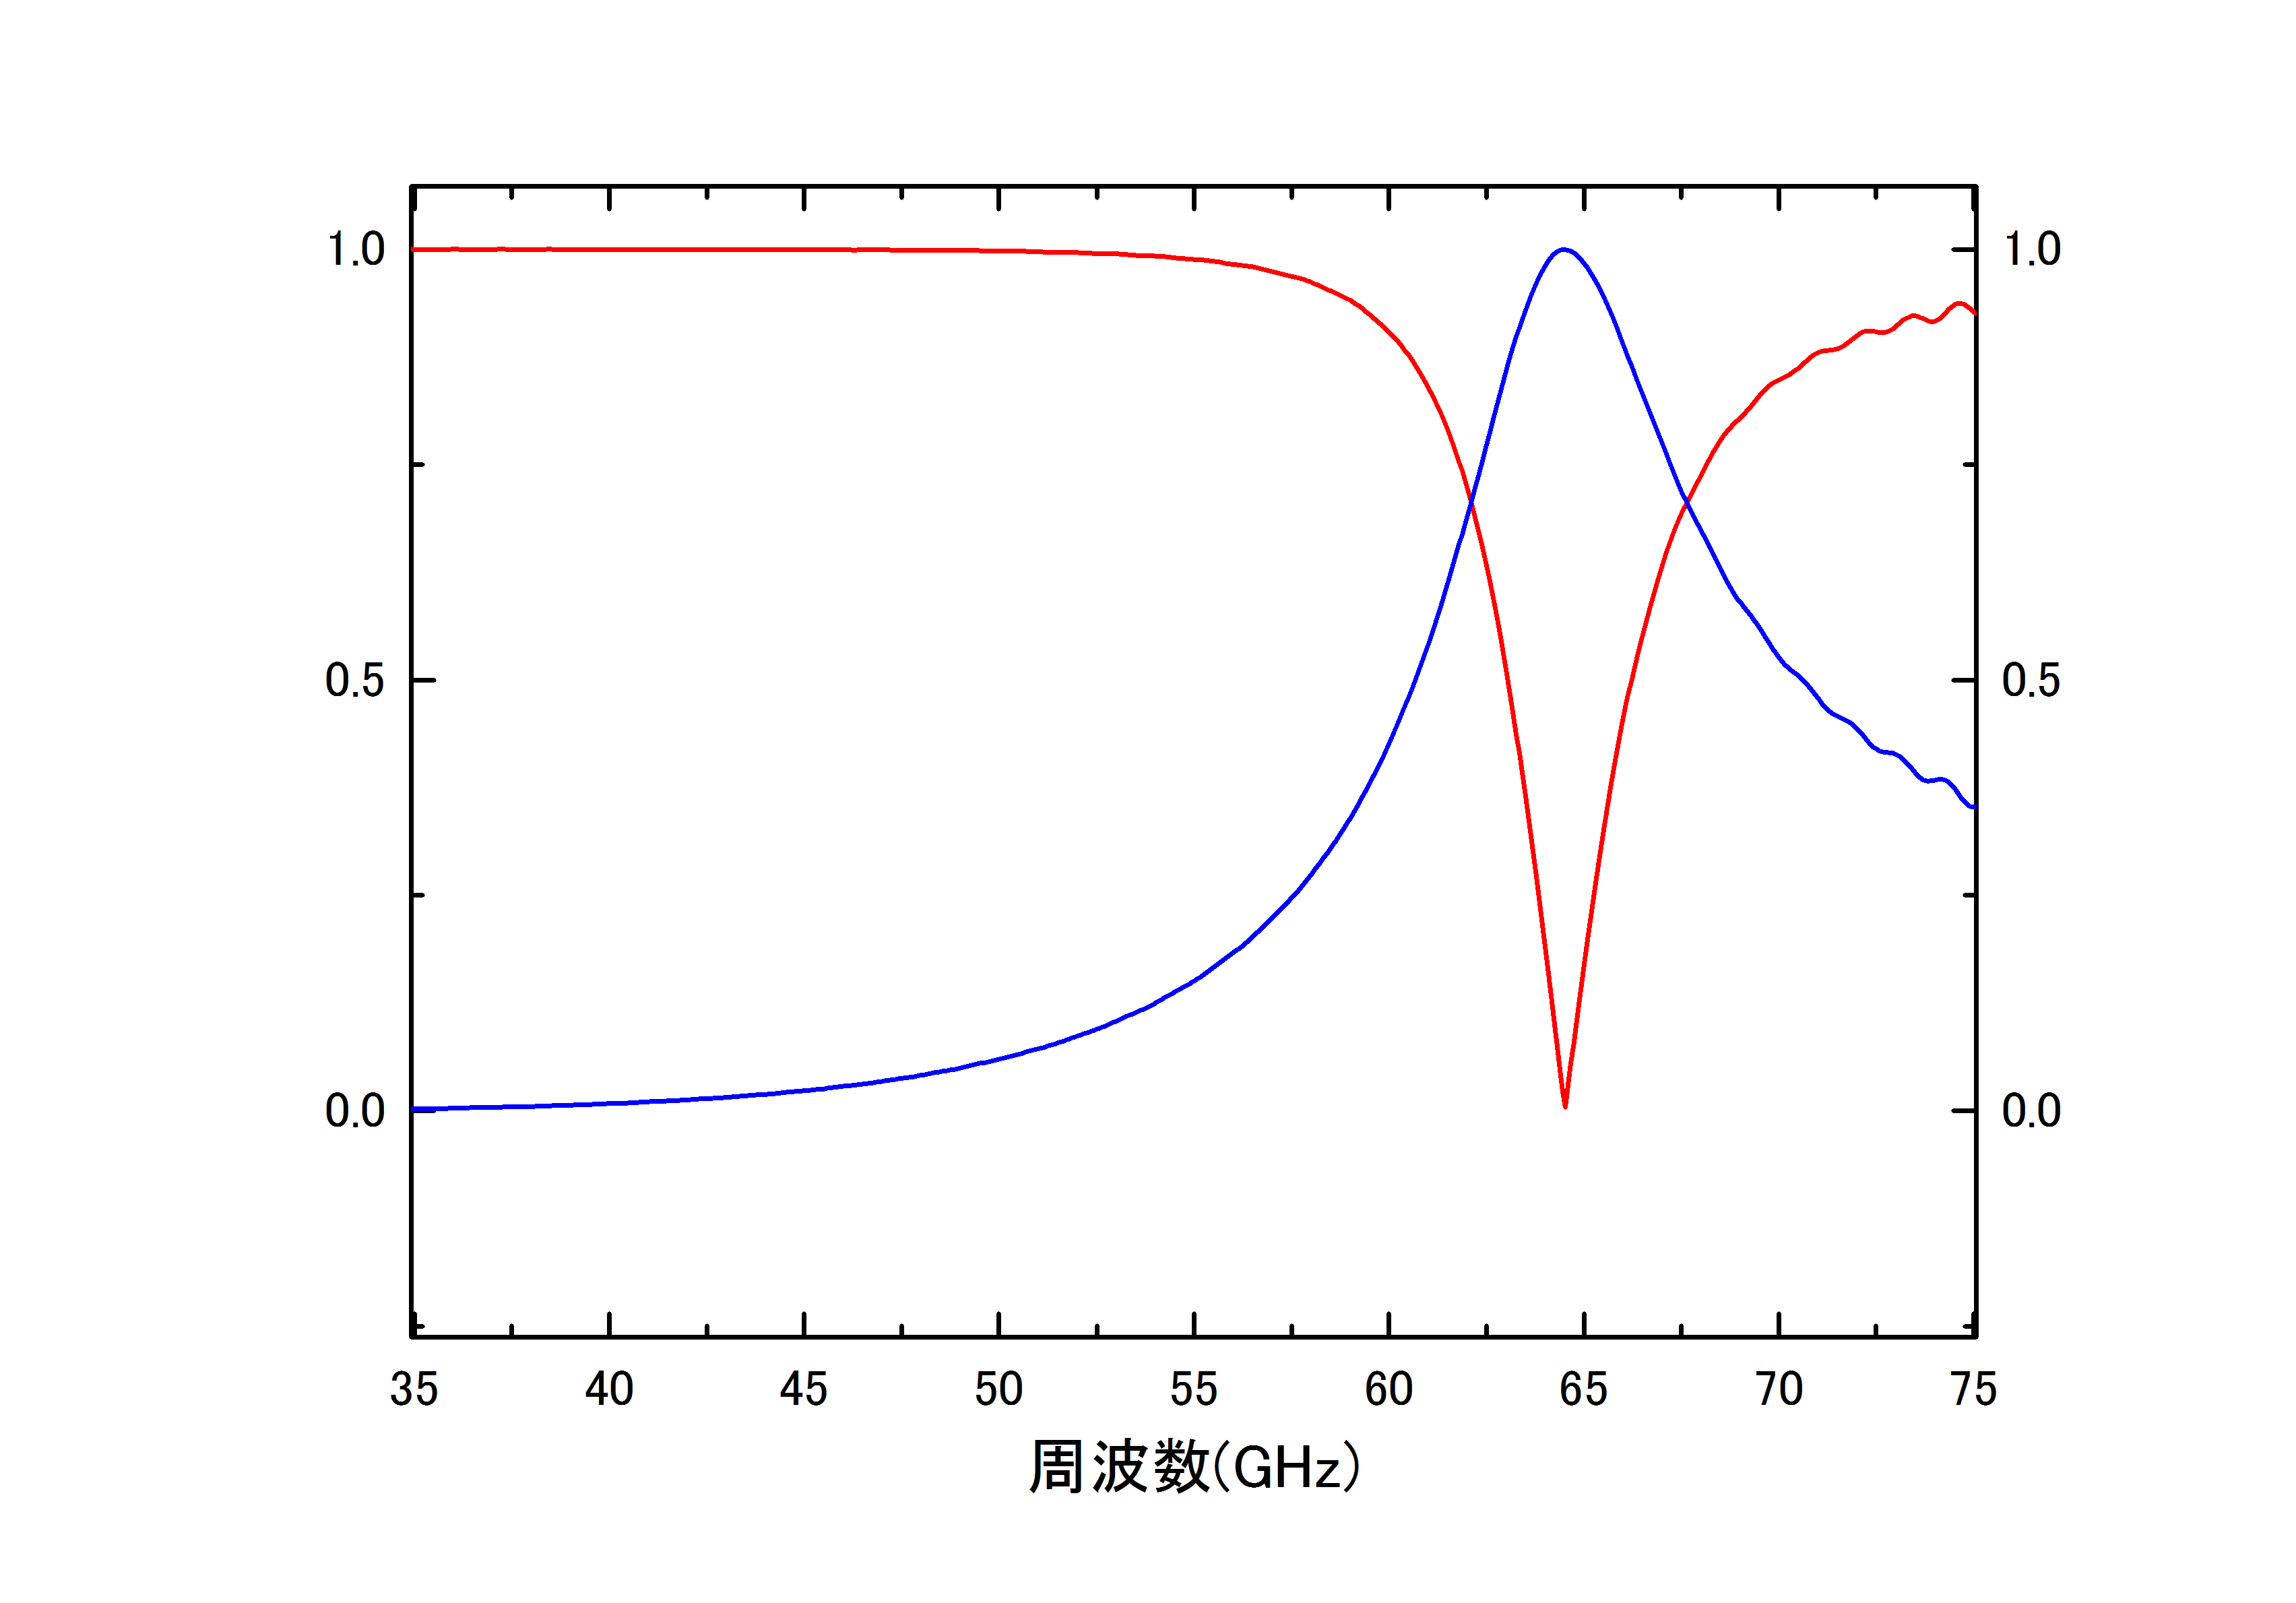
\includegraphics[width=70mm]{./image/Graph1.jpg}
  \end{center}
  \caption{S$_{11}$(赤)とS$_{21}$(青)}
  \label{fig:two}
 \end{minipage}
\end{figure}

\subsubsection{誘電体なし基板あり}
次に、共振周波数を調整するための誘電体は挿入せずに、
基板のみ共振器内部に設置した。
% 存在するモデルでシミュレーションを実行した。
% 試料が乗っている
この基板は動かさないため、
この場合の
% 値が今回得られる
共振周波数が最大値となる。
基板自体も誘電体のため、
空の場合よりも共振周波数が下がるが、
最大値として約52GHz
の共振周波数が得られた。


\begin{figure}[h]
 \begin{minipage}{0.5\hsize}
  \begin{center}
   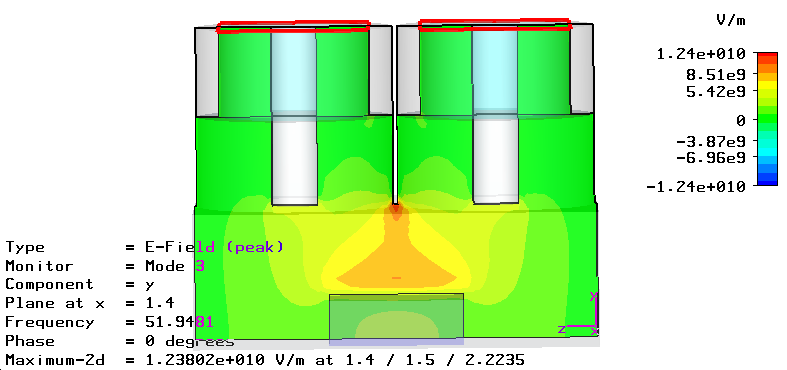
\includegraphics[width=70mm]{./image/model73_kiban_e_y_y.png}
  \end{center}
  \caption{E$_y$の空間分布}
  \label{fig:one}
 \end{minipage}
 \begin{minipage}{0.5\hsize}
  \begin{center}
   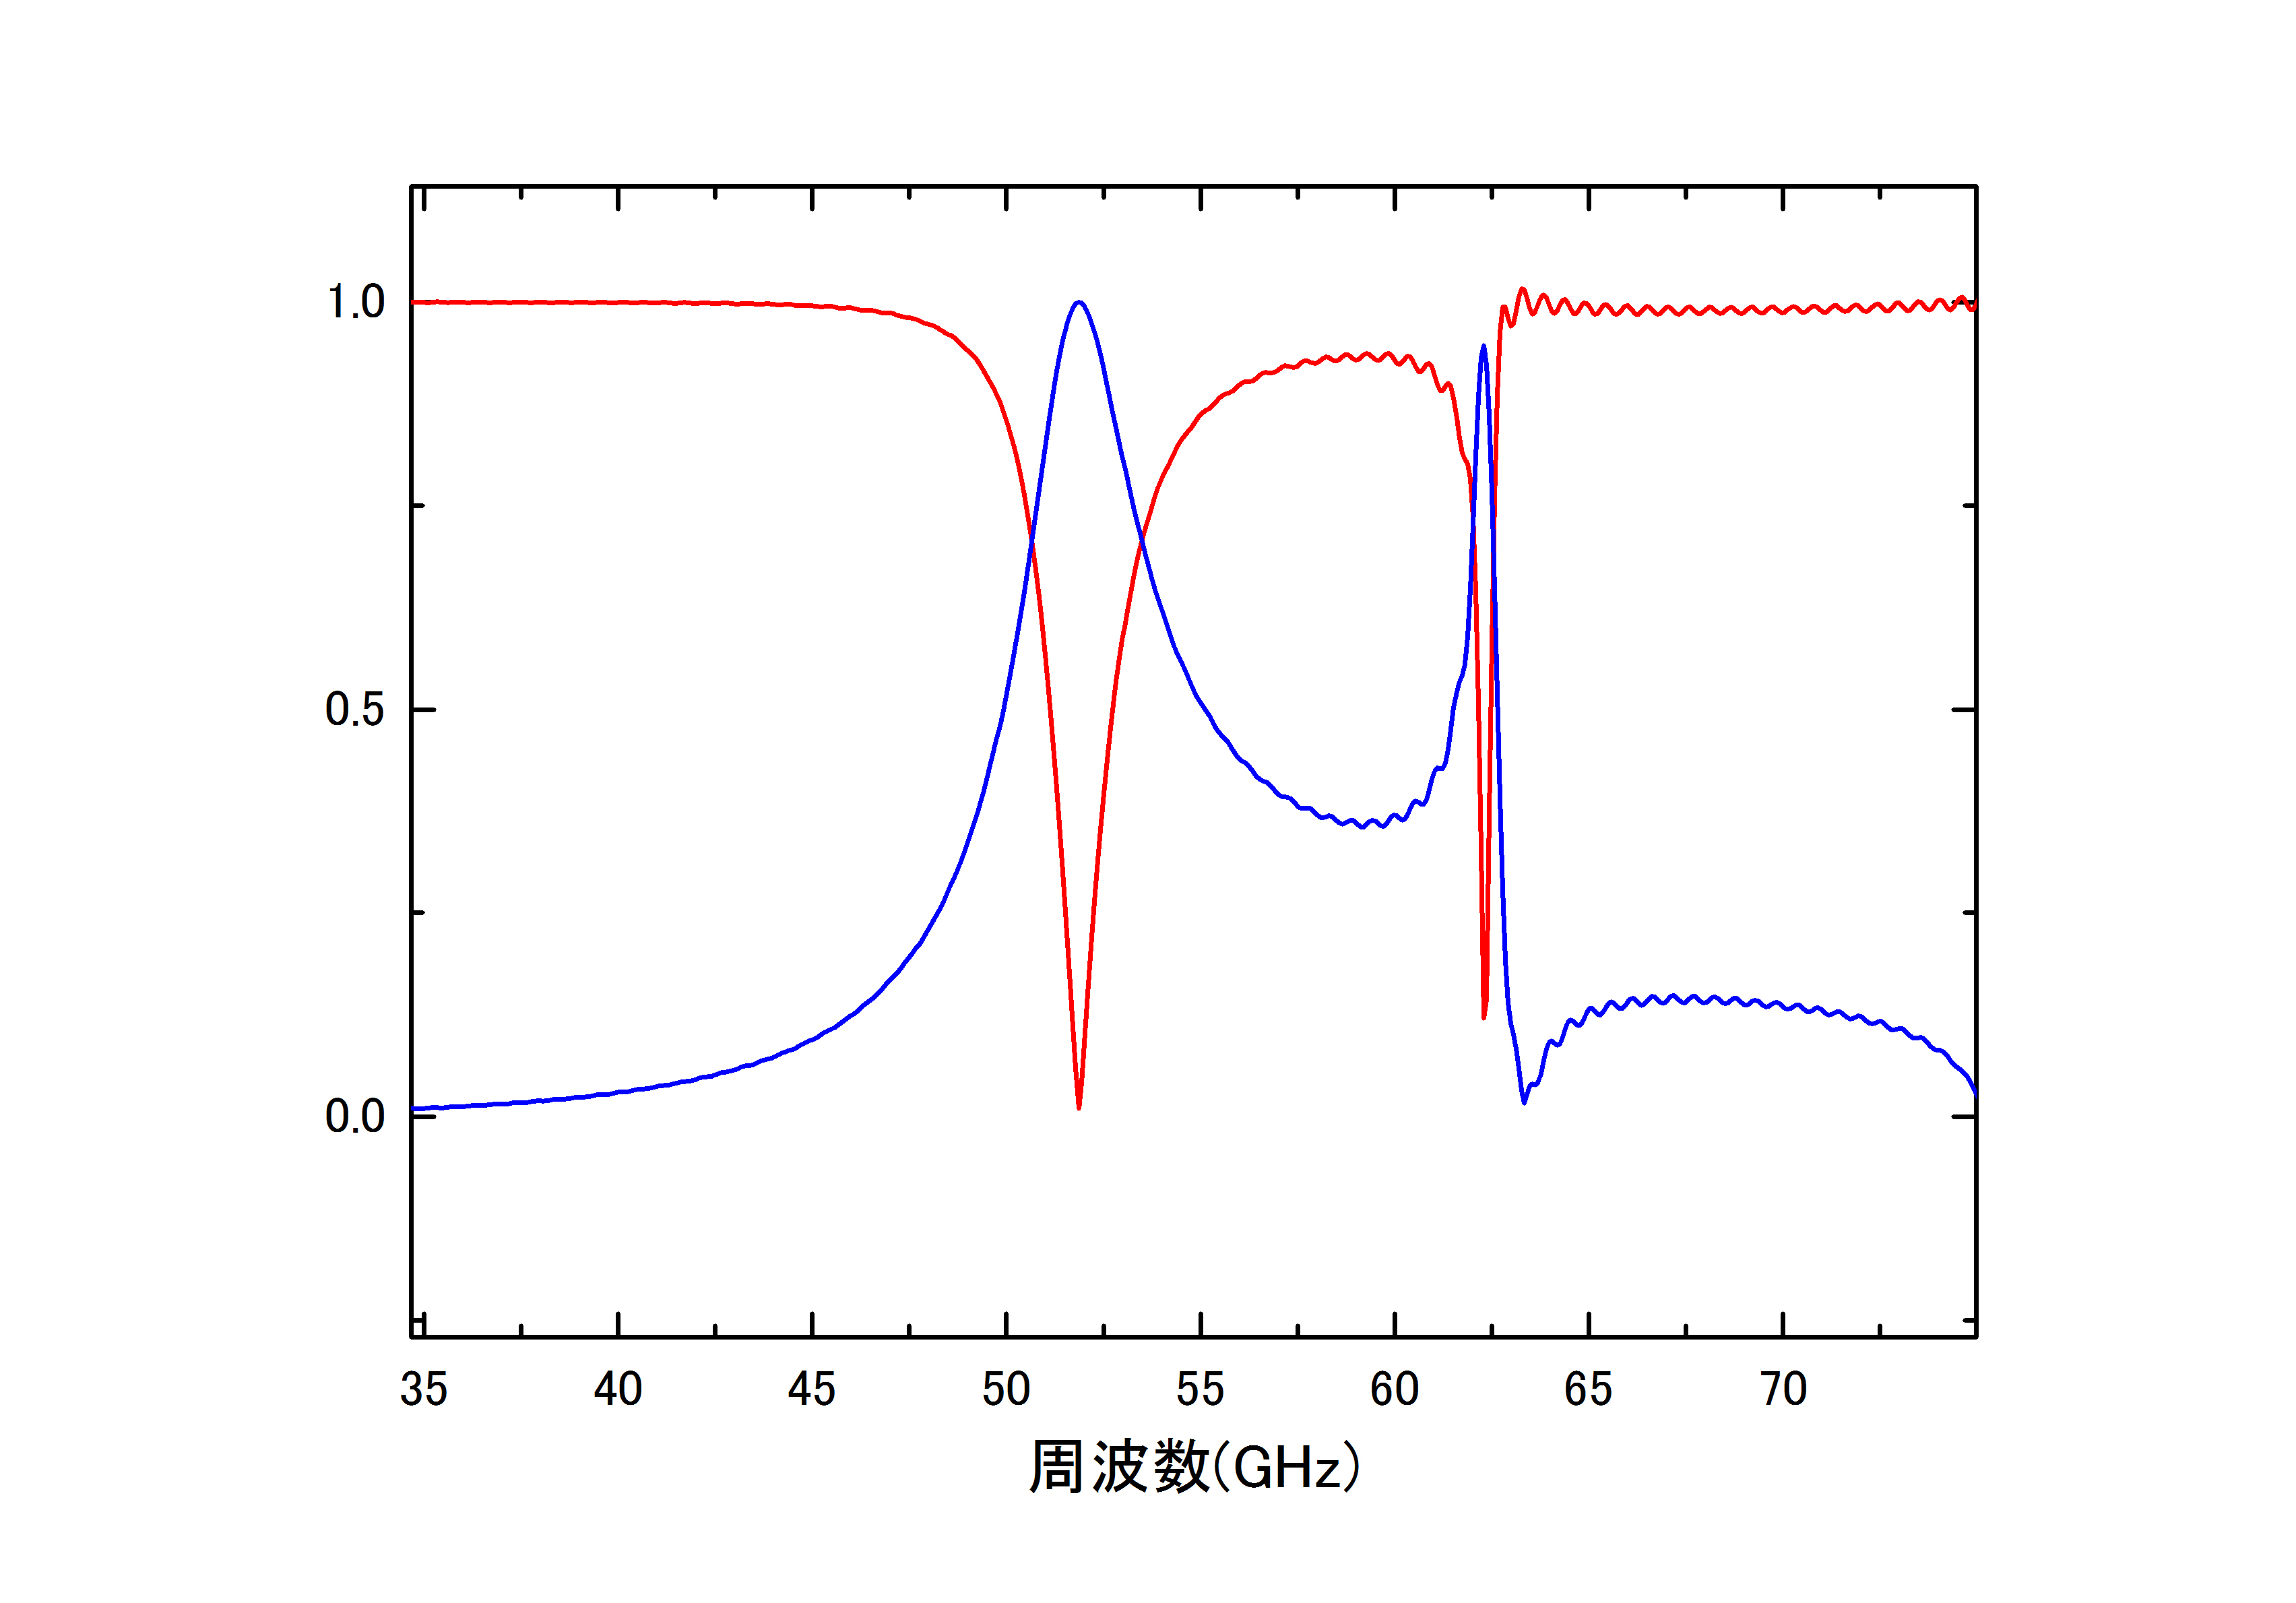
\includegraphics[width=70mm]{./image/Graph5.jpg}
  \end{center}
  \caption{S$_{11}$(赤)とS$_{21}$(青)}
  \label{fig:two}
 \end{minipage}
\end{figure}

\subsubsection{誘電体あり基板あり}
最後に、共振周波数を調整するための誘電体と
基板
の両方を
% をどちらも
含めたモデルで
% シミュレーションを行った。
計算した。
こ
の場合の
% れが今回得られる
共振周波数が最小値となる。
その結果、
約37GHzまで共振周波数を減少させることができた。

\begin{figure}[h]
 \begin{minipage}{0.5\hsize}
  \begin{center}
   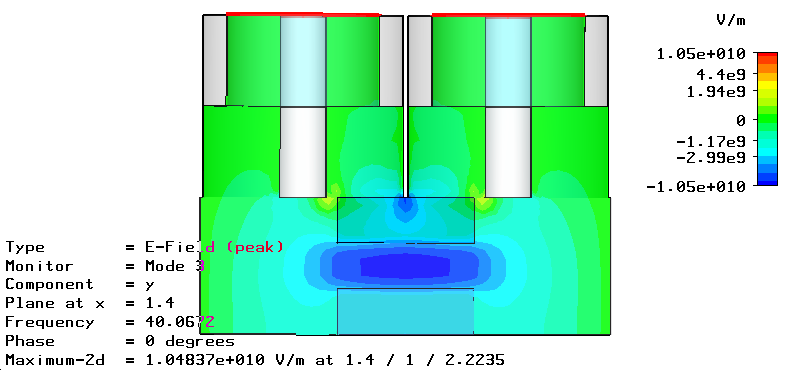
\includegraphics[width=70mm]{./image/model73_y_x.png}
  \end{center}
  \caption{E$_y$の空間分布}
  \label{fig:one}
 \end{minipage}
 \begin{minipage}{0.5\hsize}
  \begin{center}
   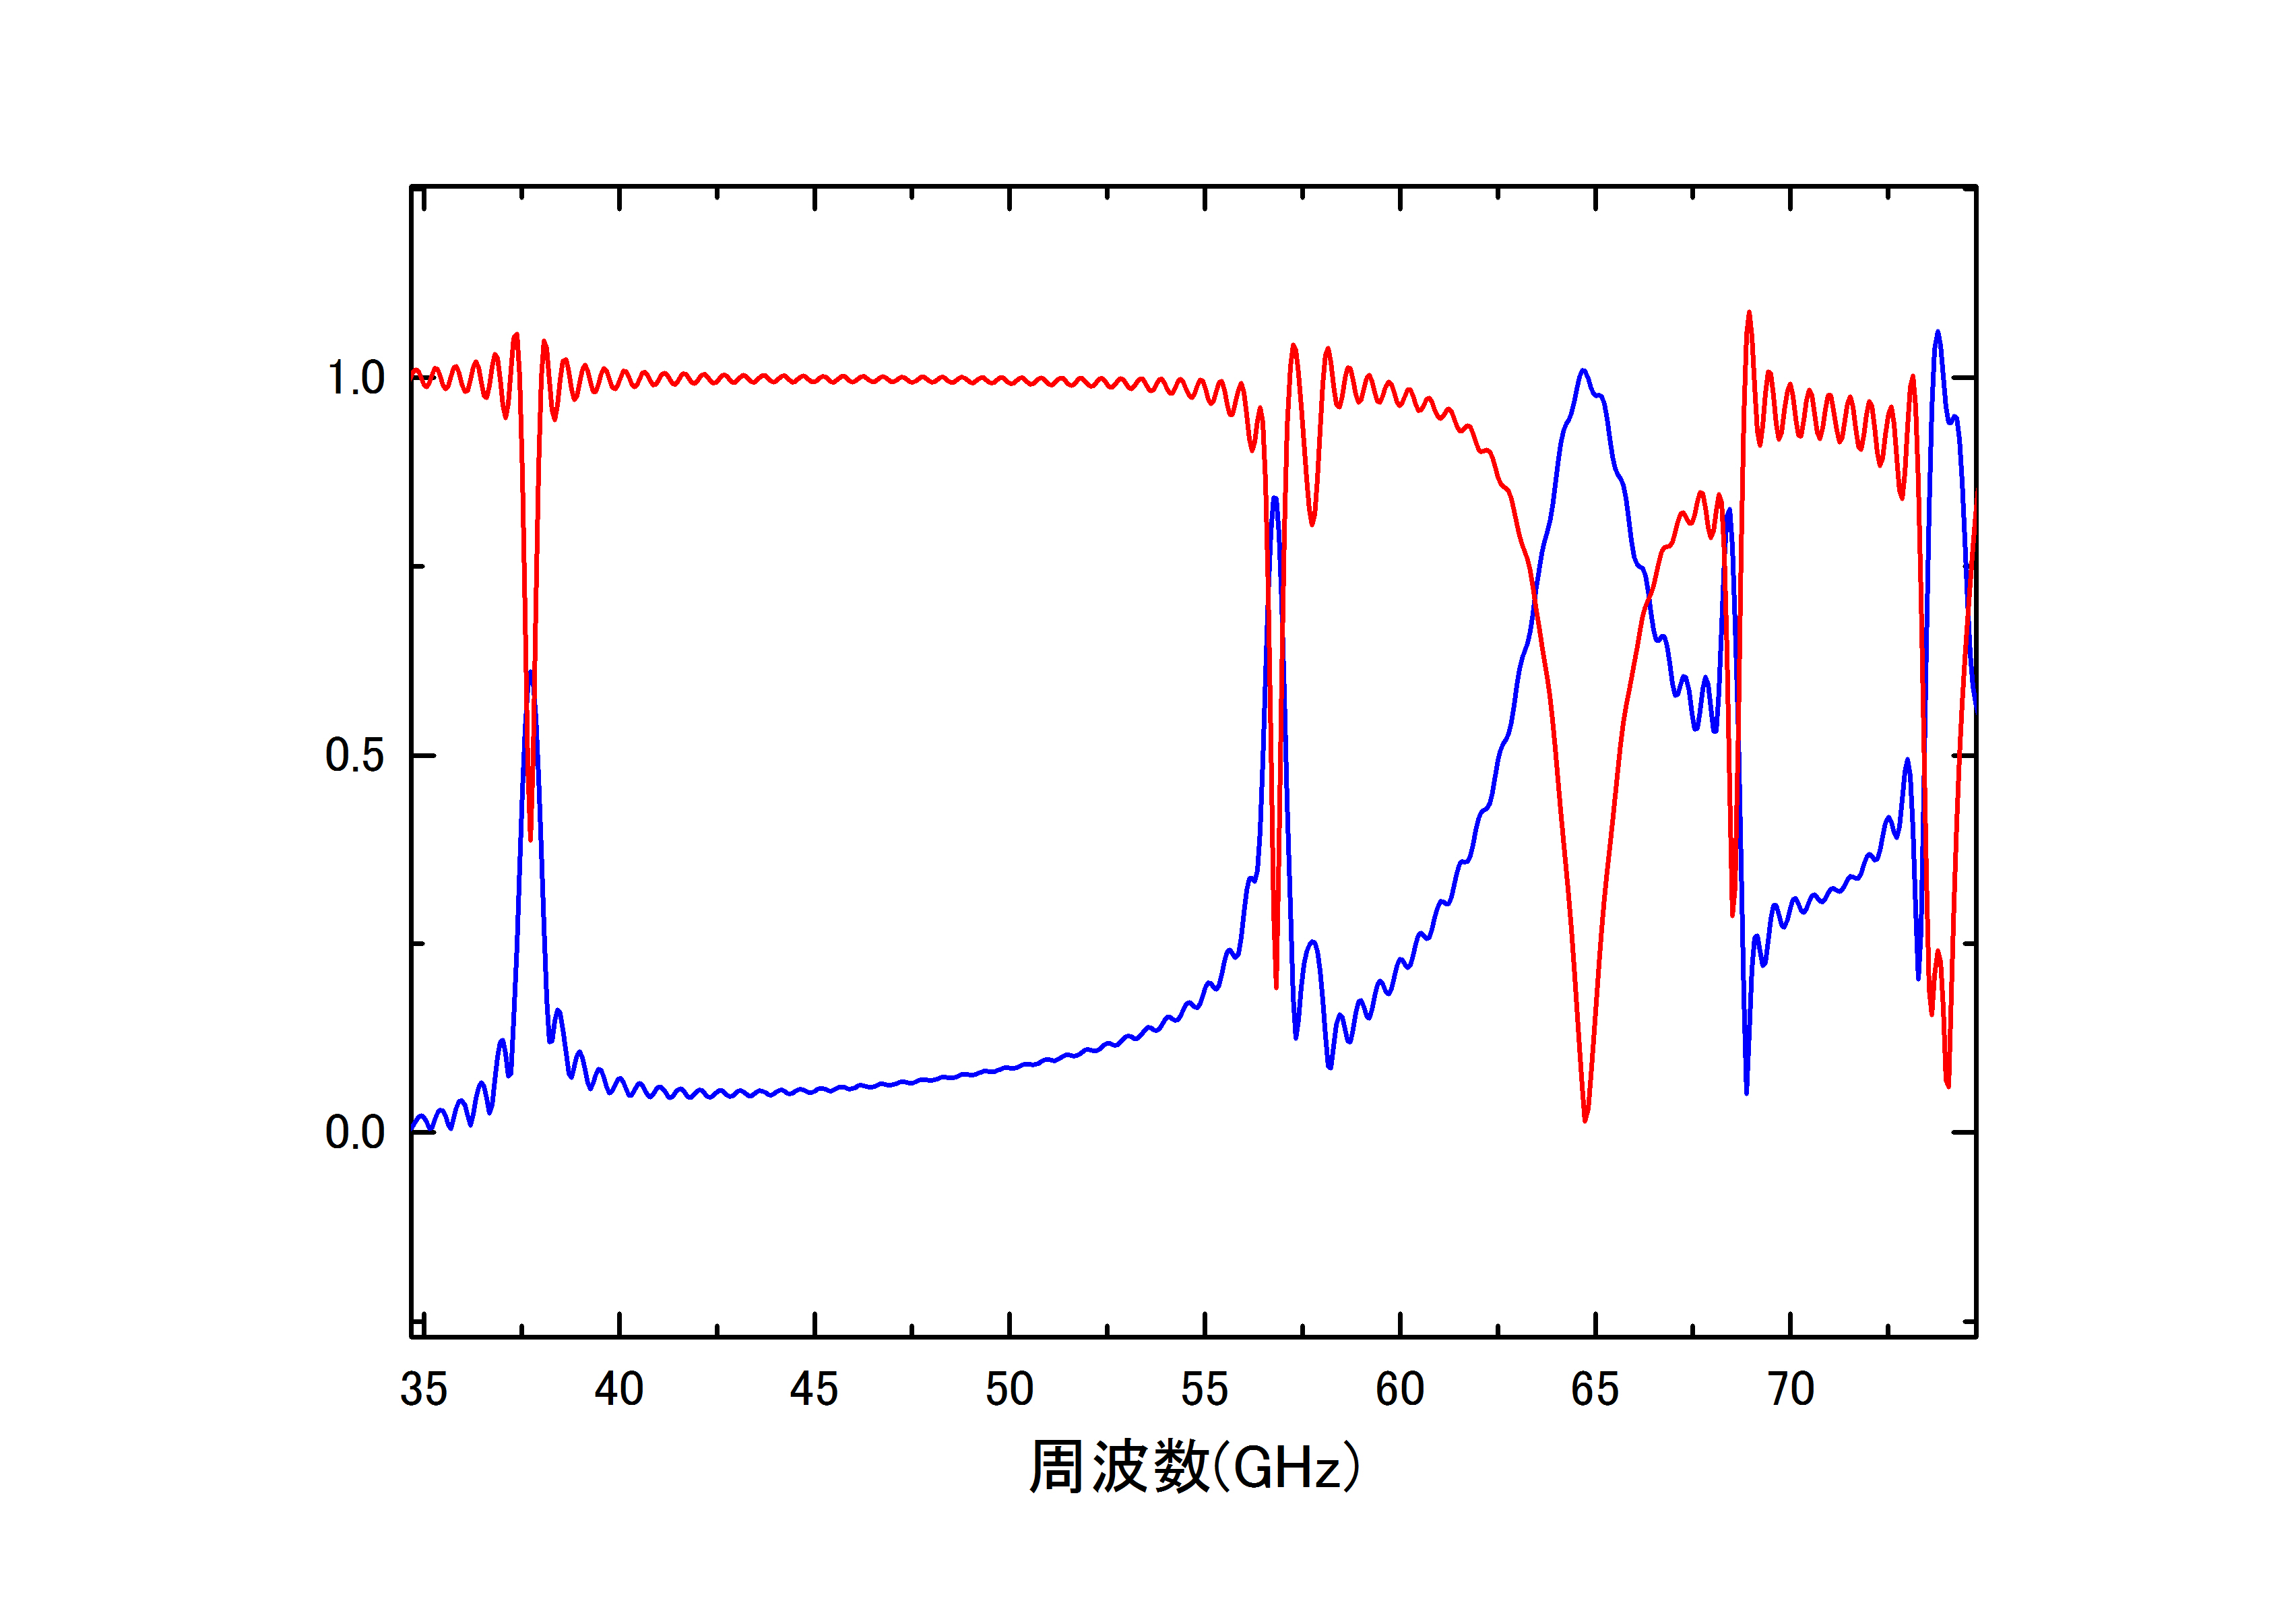
\includegraphics[width=70mm]{./image/Graph4.jpg}
  \end{center}
  \caption{S$_{11}$(赤)とS$_{21}$(青)}
  \label{fig:two}
 \end{minipage}
\end{figure}

\subsection*{誘電体挿入による共振周波数の変化}
Fig.4.14に示すように誘電体を徐々に
共振器内部へ挿入した場合の共振周波数の変化を
過渡解析で検証した。
水色の部分が共振器、青色の部分が誘電体である。
Fig.4.14に示す図では、同軸ケーブルは省略しているが
計算においては同軸ケーブルを接続したモデルで計算している。
\vspace{10 mm}

\begin{figure}[h]
  \begin{center}
    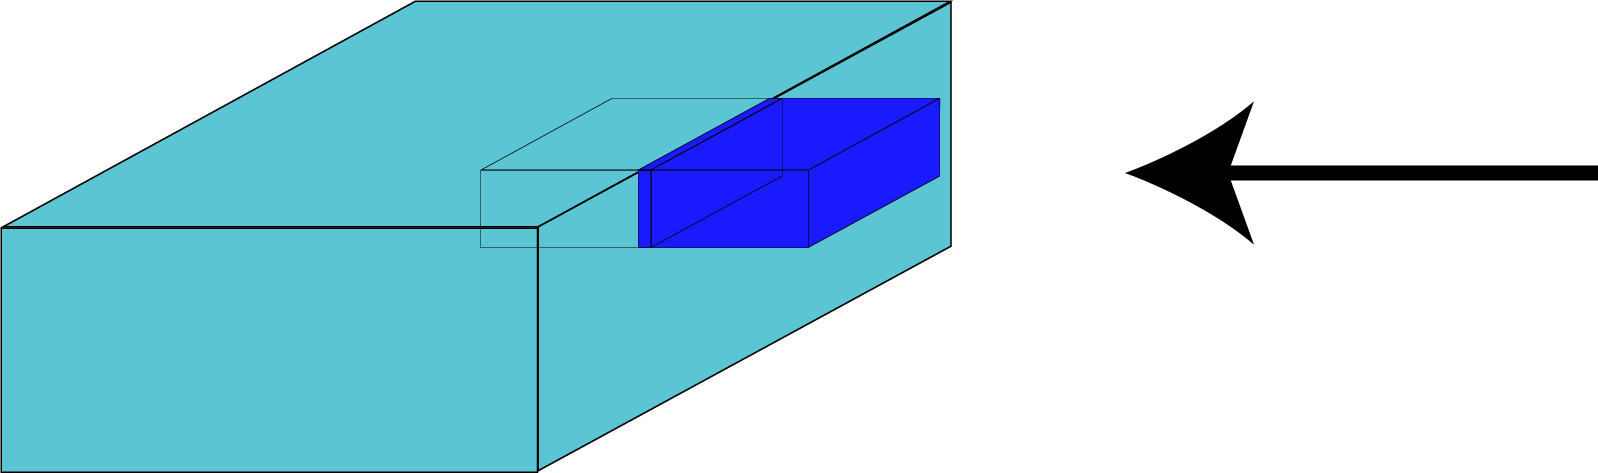
\includegraphics[width=8cm]{./image/insert.png}
    \caption{共振器への誘電体挿入}
    \label{fig:insert}
  \end{center}
\end{figure}

解析結果をFig.4.15に示す。
変分法を用いる固有値解析モードの場合、
共振周波数の低い順に共振モードをリストアップするため、
誘電体挿入と共に固有モードの数が変わったり
% しまい、モードを共振周波数の低い順に、順番で判断する固有値解析モードでは
様々なモードが
% 混じってしまうため、
入れ替わったりすると、共振モードの同定が難しくなる。
このため、本研究では
過渡解析のSパラメータ計算の結果Fig.4.16を利用した。
その結果からTE$_{101}$モードの共振ピークと判断出来る点を取り出し、
% プロットした。
Fig.4.15のプロットを得た。

\vspace{10 mm}

\begin{figure}[h]
  \begin{center}
    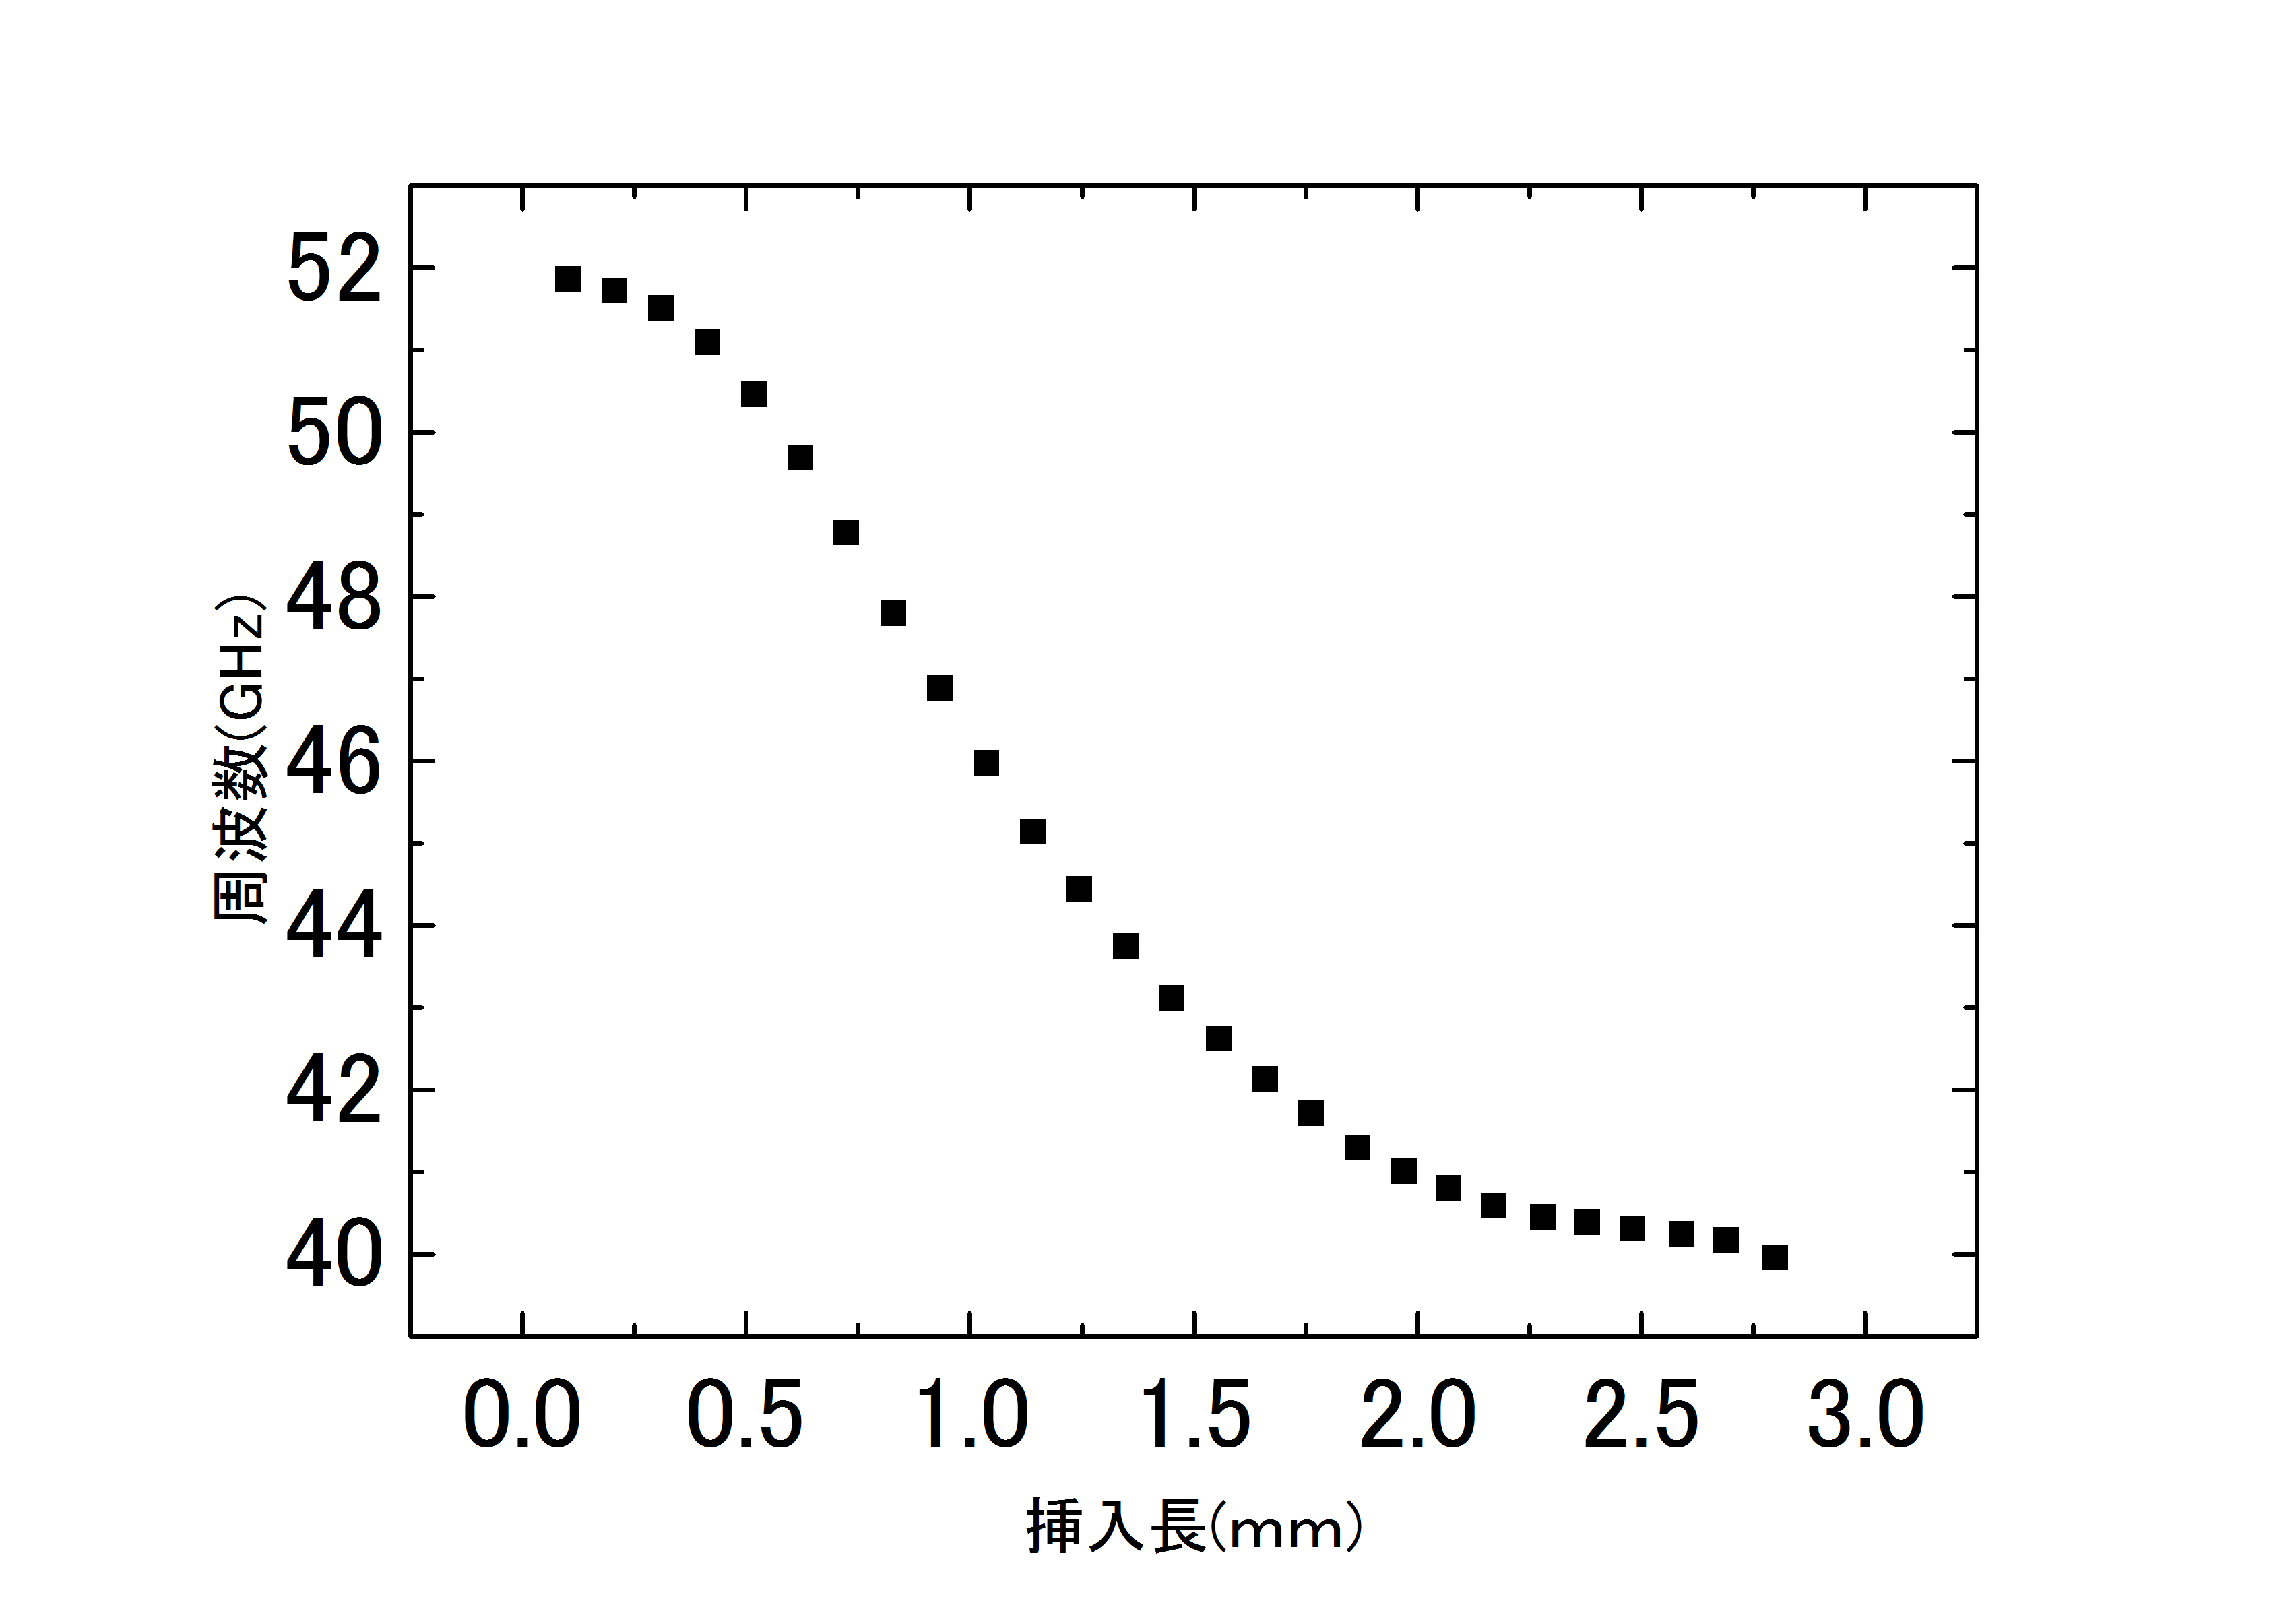
\includegraphics[width=12cm]{./image/plot2.jpg}
    \caption{誘電体挿入の際の共振周波数の変化}
    \label{fig:result}
  \end{center}
\end{figure}

\begin{figure}[h]
  \begin{center}
    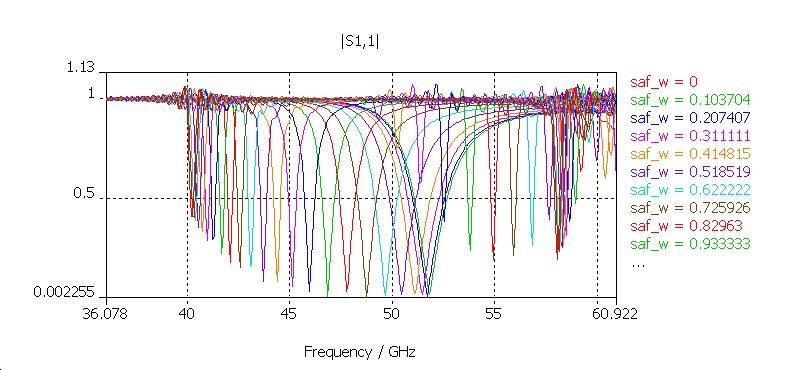
\includegraphics[width=16cm]{./image/sweepS11.jpg}
    \caption{過渡解析のS$_{11}$計算結果}
    \label{fig:result}
  \end{center}
\end{figure}

この結果から、誘電体挿入に伴い、
40〜52 GHzの周波数範囲で共振周波数
% が変化する様子が観測できた。
を調整できることが確認できた。
また、過渡解析
% の結果であるので、
モードでFig.4.16の示すSパラメータの共振曲線が得られていることから、
外界との電磁場結合も保証する
% きちんと共振が起こる
モデルであることがわかる。


% \subsection*{考察}
%
% あああああああああああああああ
% あああああああ
%
% あああああああ
% ああああ
%
% あああああああ
% ああああ
%
% あああああああああああああああ
% あああああああ
%
% あああああああああああああああ
% あああああああ
